\chapter{Introduction to \Ejs}\label{chapter:EjsIntro}
\begin{quote}
Machines should work. People should think.  {\em Richard Hamming}
\end{quote}

This chapter provides an overview of \Ejs\ (\ejs\ for short), the high-level modeling and authoring tool that we use to make our models explicit and to run (execute) these models in order to study their behavior. In order to provide a
global perspective of the modeling process, we load, inspect, and run an existing simple harmonic oscillator
simulation. We then modify the simulation to show how \ejs\ engages the user in the modeling process and greatly
reduces the amount of programming required to implement an idea.

% ------------------------
  \section{About \Ejs}
% ------------------------

Computer modeling is intimately tied to computer simulation.  The modeling cycle requires (1) a description and an analysis of
the problem, (2) the identification of variables and the algorithms, (3) implementation on a specific hardware-software
platform, (4) execution of the implementation and analysis of the results, (5) refinement and generalization, and (6)
presentation of results. A computer simulation is an implementation of a model (a program) that allows us to performing experiments on that
model with different initial conditions with the objective of learning about the behavior of the
model.\index{Simulation} Of course, the applicability of the results of the simulation to those of the real (physical)
system depends on how well the model describes reality.\index{Simulation!Model} The process of devising broader and
more accurate models is basically what science is about.

The implementation of a model and the visualization of its output require that we learn to program the computer. Programming is a fascinating experience, because it gives us complete control of every visual and numeric detail of the simulated world. But it is also a technical task which can intimidate people without an extensive background in computer science. This needs not be the case if we use the appropriate tool. \Ejs\ is an authoring tool that has been designed to allow scientists (not only computer scientists!) to create simulations in Java. \ejs\ simplifies this task, both from the technical and from the conceptual point of view.

\ejs\ provides a simple yet powerful conceptual structure for building simulations. The tool offers a left-to-right
sequence of workpanels which the author uses to implement the model and its graphical user interface. \ejs\ automates technical tasks such as numerically solving ordinary differential equations, \index{ODE} event-handling (see chapter~\ref{ref:chapter:Events}), and multithreading (using Java threads) for animation. The low-level communication between the program and the end-user that takes place at run-time, including handling of mouse actions within the simulation's graphical interface, is accomplished without low-level programming.

Obviously, part of the task still depends on us. We are responsible for providing a model for the phenomenon and for
designing and selecting an output view that shows the model's main features. These high-level tasks are more related to
science than to computer programming. We are encouraged to devote our time and energy studying the science we are
interested in, something that the computer cannot do. The purpose of this chapter is to demonstrate that this is not
only possible but can actually be relatively easy, with the help, of course, of \Ejs.

% ------------------------
    \section{Installing and Running the Software}\label{section:02Installation}\index{\Ejs!installing and running}
% ------------------------

Let us begin by installing \Ejs\ in a computer and running it. \ejs\ is a Java program that can be run under any
operating system that supports a Java Virtual Machine (VM). Because Java is designed to be platform independent, the
\ejs\ user interface on Apple OS X, UNIX, and Linux is almost identical to the Windows interface shown in this book.

To install and run \ejs, do the following:

\begin{numberlist}

\item \textbf{Install the Java Runtime Environment.} \ejs\ requires the Java Runtime Environment (JRE), version 1.5 or later.
The JRE may already be installed in your computer, but, if this is not the case, use the copy provided on the CD that
comes with this book or, even better, visit the Java site at \link{http://java.sun.com} and follow instructions there
to download and install the latest version available.

\item \textbf{Copy \ejs\ to your hard disk.} You'll find \ejs\ in a compressed ZIP file called \file{Ejs.zip} on the CD of the book.
Uncompress this file anywhere in your computer's hard disk to create a directory called \file{Ejs}. This directory
contains everything that is needed to run \ejs.~\footnote{In Unix-like systems, the \file{Ejs} directory may be
uncompressed as read-only. Please enable write permissions for the \file{Ejs} directory and all its subdirectories.}

\item \textbf{Run the \ejs\ console.} Inside the newly-created \file{Ejs} directory, you will find a file called
\file{EjsConsole.jar}.\index{jar files!EjsConsole.jar}\index{Easy Java Simulations!console} Double-click it to run the
\ejs\ console shown in Figure~\ref{fig:02EjsIntro/EjsConsole}.
\note{If double-clicking doesn't run the console, open a
system terminal window, change to the \file{Ejs} directory, and type the command: \code{java -jar EjsConsole.jar}.
You'll need to fully qualify the \code{java} command if it is not in your system's PATH.}

\begin{figure}[htb]
  \centering
  \subfigure{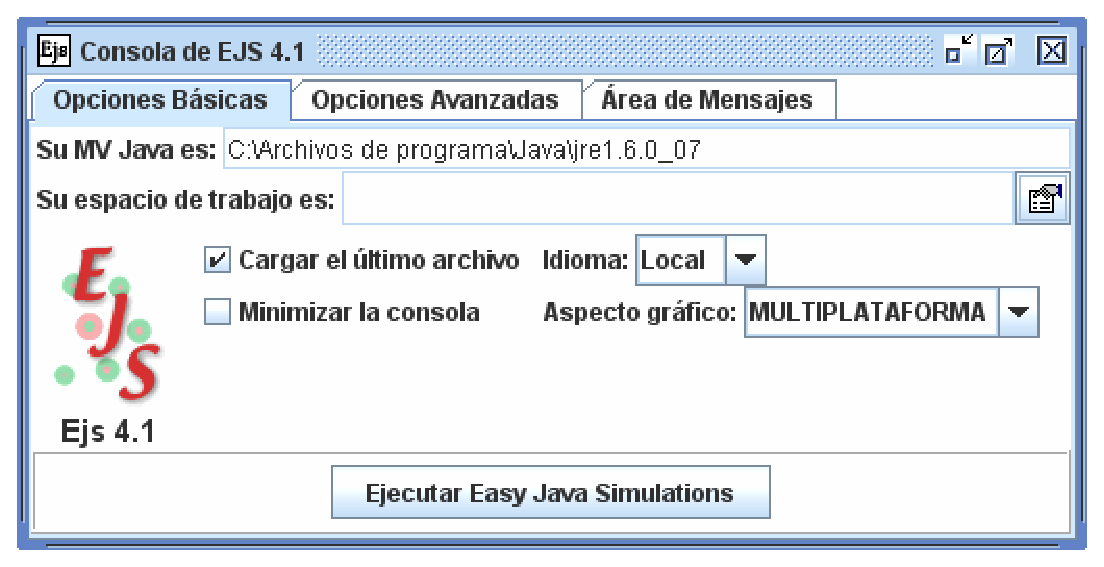
\includegraphics[scale=\scale]{02EjsIntro/images/EjsConsole1.eps}}
  \subfigure{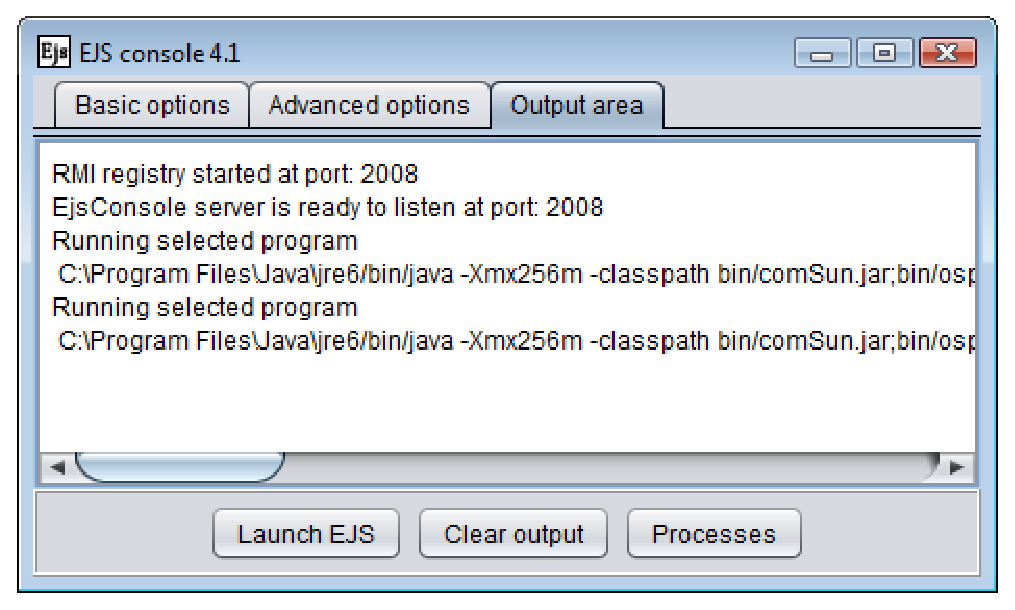
\includegraphics[scale=\scale]{02EjsIntro/images/EjsConsole2.eps}}
  \caption{Two views of the \ejs\ console. The second view is what you will see after double-clicking the \file{EjsConsole.jar} file.}
  \label{fig:02EjsIntro/EjsConsole}
\end{figure}

\end{numberlist}

You should see the console (Figure~\ref{fig:02EjsIntro/EjsConsole}) in your computer screen. The console is not part of
\ejs\ itself, but a utility to launch one or several instances (copies) of \ejs\ and to perform other \ejs-related
tasks.  The console is important because it displays \ejs\ program information and error messages and we refer to it
from time to time in this book. The default console configuration creates an instance of \ejs\ which should appear in
your screen. Other console features, such as its ability to process collections of \ejs\ models, are described in the
appendices.

Study the structure of the installation directory before proceeding with \ejs\ modeling. \index{\Ejs!directory
structure} The \file{Ejs} directory contains the single file \file{EjsConsole.jar} which you used to run \ejs\ and two
directories called \file{data} and \file{Simulations}. The \file{data} directory contains the program files for \ejs,
and should not be modified. The second directory, \file{Simulations}, is your working directory and contains the
following important subdirectories:
\begin{bulletlist}
  \item \file{\_apps} is the (initially empty) directory where \ejs\ places files generated when a simulation is run.
  \item \file{\_config} contains configuration files that enable a user to customize the interface.
  \item \file{\_library} contains the common library that is required by all \ejs\ simulations.
\end{bulletlist}
\noindent \ejs\ creates new files or use files already in these subdirectories as you run models and it is important that you do not
delete, move, or rename these subdirectories. You will find other subdirectories within \file{Simulations} that begin
with the underscore character \lit{\file{\_}}. These directories contain sample simulations. In particular, the
\file{\_ModelingScience} directory includes the \ejs\ models described in this book.

We are now ready to turn our attention to the \ejs\ modeling tool, displayed (with annotations) in
Figure~\ref{fig:02EjsIntro/EjsInterface}. Despite its simple interface, \ejs\ has all the tools needed for a complete
modeling cycle.

\begin{figure}[htb]
  \centering
  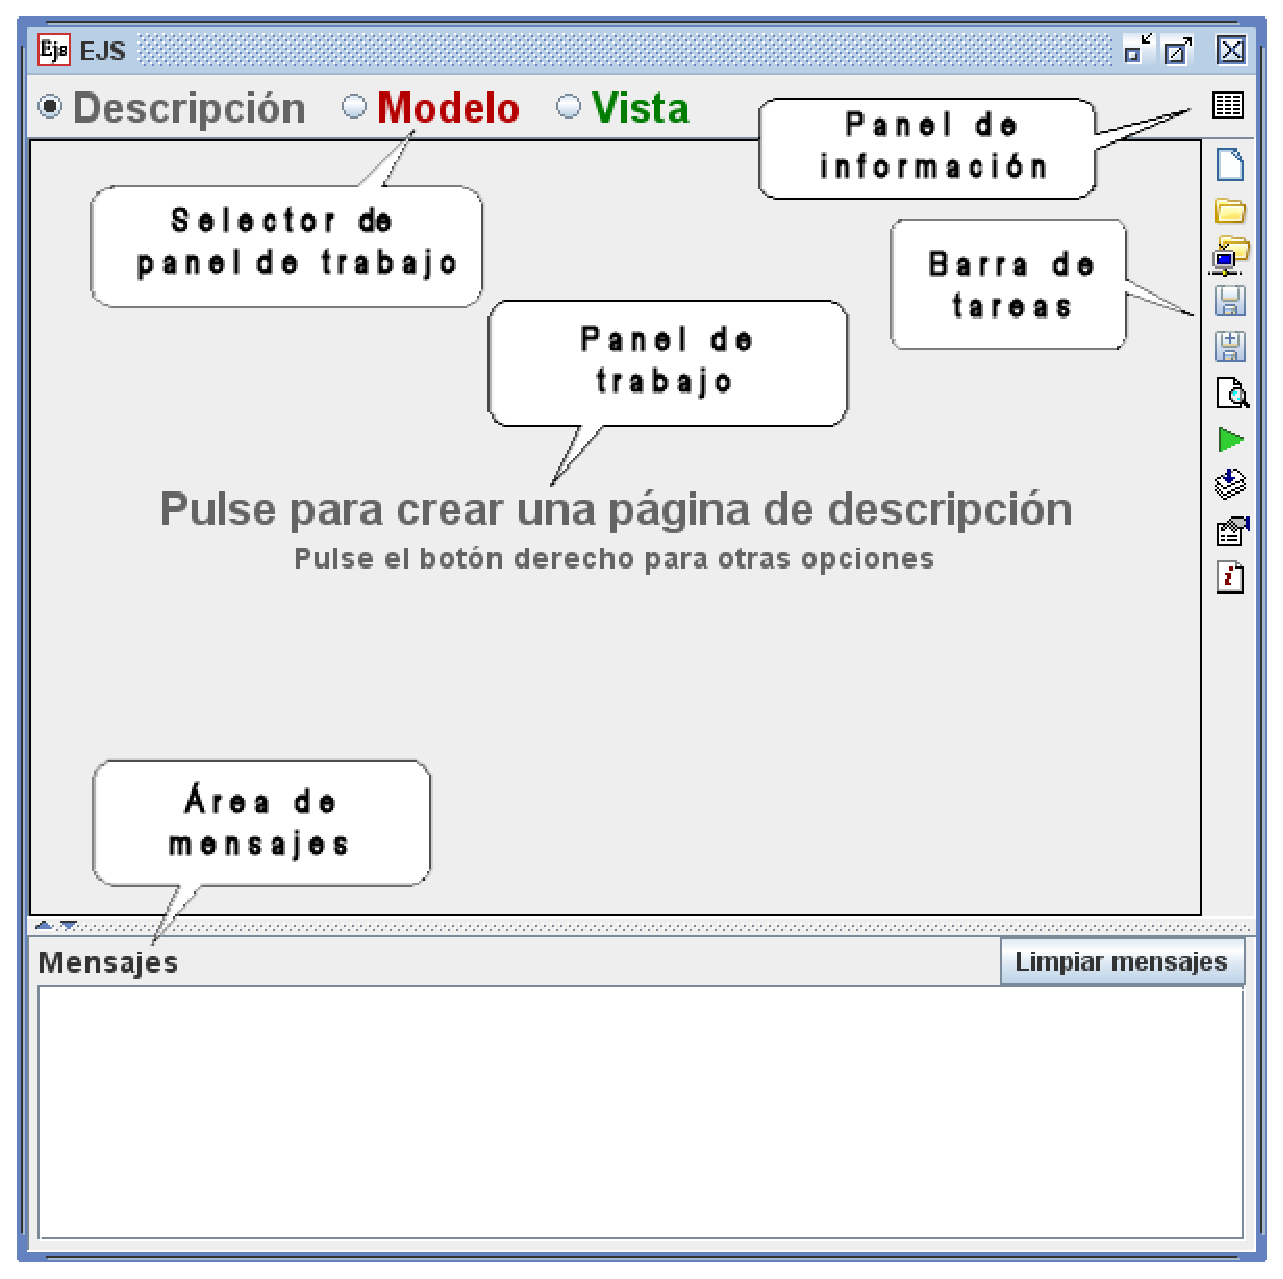
\includegraphics[scale=\scale]{02EjsIntro/images/EjsInterface.eps}
  \caption{The \Ejs\ user interface with annotations.}
  \label{fig:02EjsIntro/EjsInterface}
\end{figure}

The taskbar\index{\Ejs!taskbar} to the right of the window provides a series of icons with the standard operations to
clear, open and save a file, configure \ejs, and display program information and help. It also provides icons to run a
simulation and to package one or more simulations in a jar file.  Right-clicking on taskbar icons invokes alternative (but related) actions that will be described as needed. The bottom part of the interface contains an output area\index{\Ejs!output area} where \ejs\ prints informational messages. Finally, the central part of the interface contains the workpanels where the modeling is done.

\Ejs\ provides three workpanels for modeling. The first panel, called \lit{Description}, allows us to create and edit multimedia HTML-based narrative that describes the model.\index{HTML}  Each narrative page appears in a tabbed pane within the
workpanel and right-clicking on the tab allows the user to edit the narrative or to import additional narrative. The second workpanel, labeled \lit{Model}, is dedicated to the modeling process. We use this panel to create variables that describe the model, to initialize these variables, and to write algorithms that describe how this model changes in time. The third workpanel is called \lit{View} and is dedicated to the task of building the graphical user interface that allows users to control the simulation and to display its output. We do this by selecting elements from palettes and adding them to the model's \lit{Tree of Elements}. For example, the \lit{Interface} palette contain buttons, sliders, and input fields and the \lit{2D Drawables} palette contains elements to plot 2D data.

% ------------------------
    \section{Inspecting the Simulation}\label{section:02Inspecting}\index{\Ejs!inspecting a simulation}
% ------------------------
In order to understand how the \lit{Description}, \lit{Model}, and \lit{View} work together, we inspect and run an
already existing simulation. Screen shots are no substitute for a live demonstration and you are encouraged to follow along on your computer as you read.

\begin{figure}[htb]
  \centering
  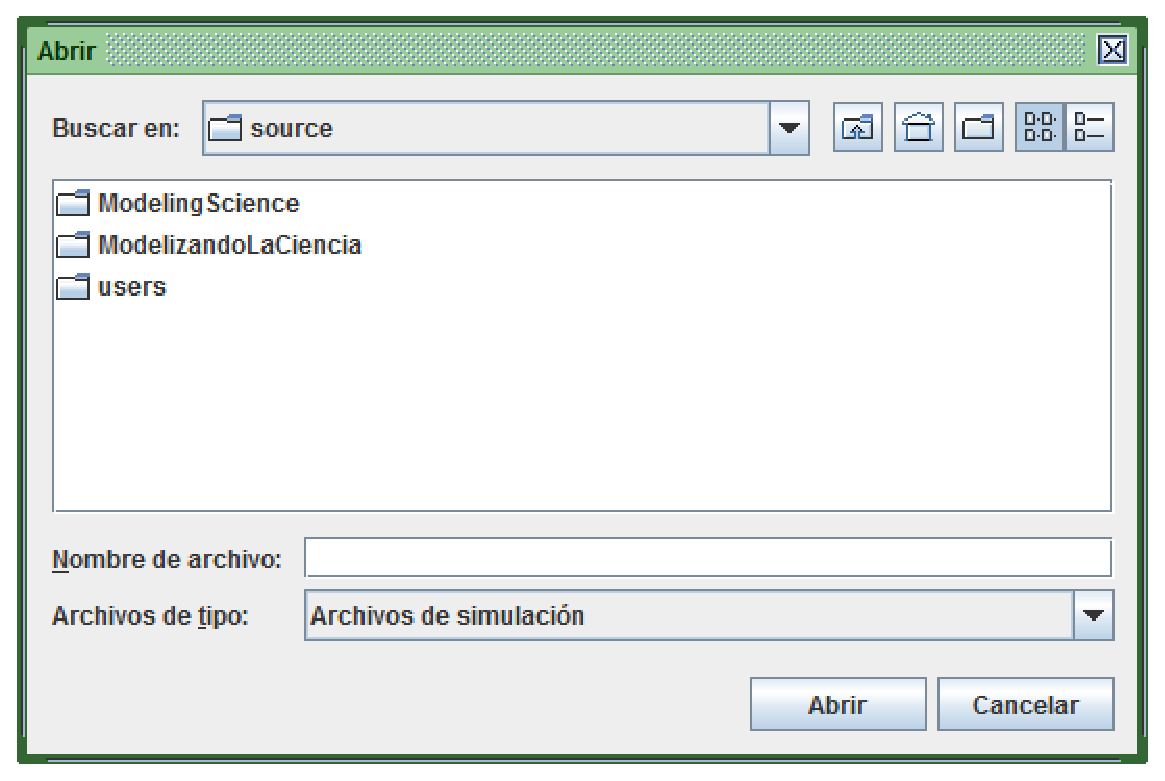
\includegraphics[scale=\scale]{02EjsIntro/images/OpenDialog.eps}
  \caption{The open file dialog lets you browse your hard disk and load an existing simulation.}
  \label{fig:02EjsIntro/OpenDialog}
\end{figure}

Click on the \lit{Open} icon,  \includegraphics[scale=\linescale]{images/open.eps}, of \ejs' taskbar. A file dialog
similar to that in Figure~\ref{fig:02EjsIntro/OpenDialog} appears showing the contents of your \file{Simulations}
directory. Go to the \file{\_ModelingScience} directory, and open the \file{02EjsIntro} subdirectory. You will find a
file called \file{MassAndSpring.xml} inside this directory. Select this file and click on the \lit{Open} button of the
file dialog.

Now, things come to life! \ejs\ reads the \file{MassAndSpring.xml} document which populates the workpanels and two new ``Ejs windows'' appear in your screen as shown in Figure~\ref{fig:02EjsIntro/SpringInterface}. A quick warning.  Don't try to interact with these windows as they are only mock-ups that help the author design the view of the
simulation. You can drag an object within a mock-up window but this will set a model's initial conditions and it is usually better to set initial conditions using a table of variables as described in Section~\ref{section:02Model}.

\begin{figure}[htb]
  \centering
  \subfigure{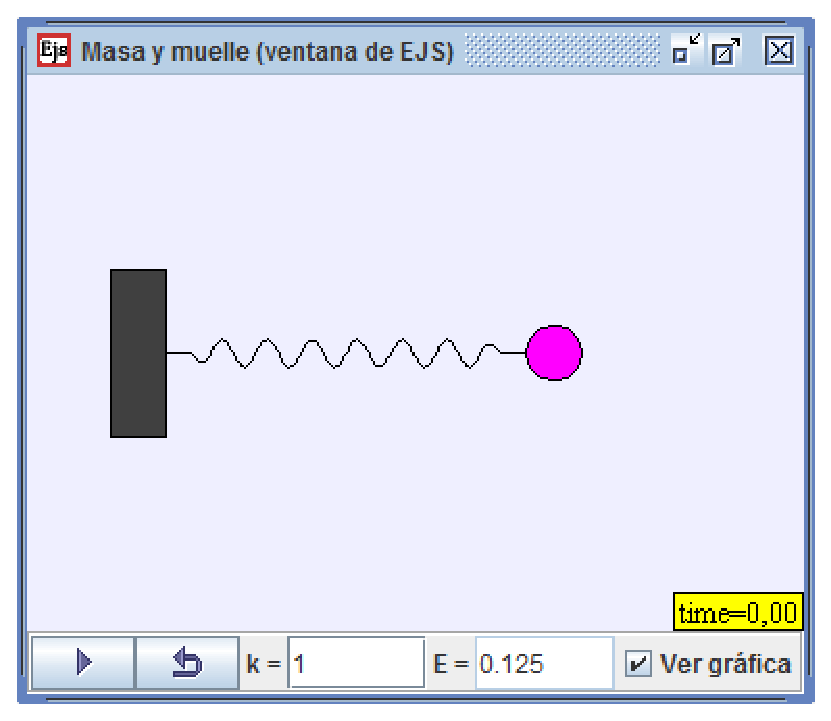
\includegraphics[scale=\scale]{02EjsIntro/images/SpringInterface1.eps}}
  \subfigure{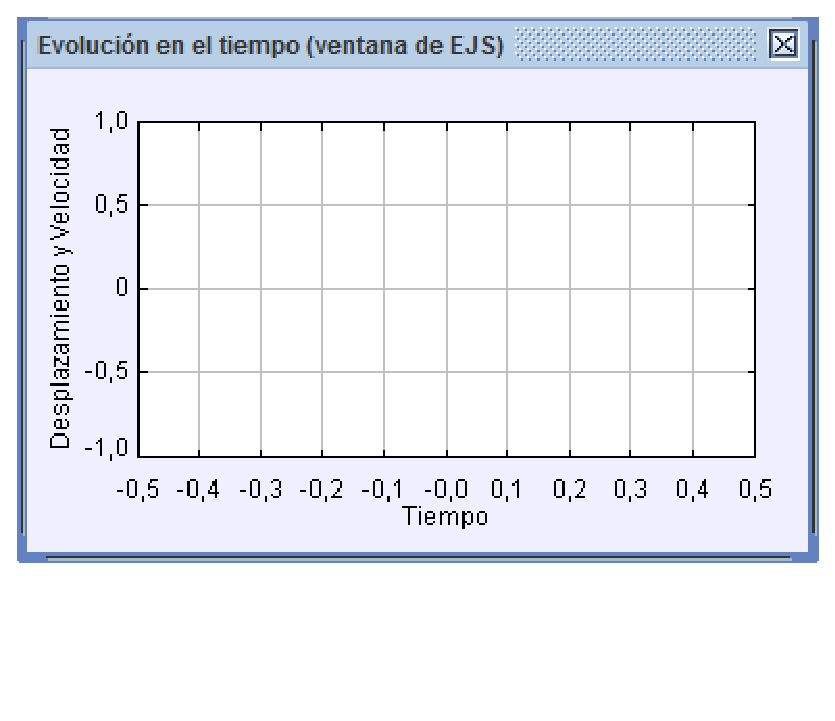
\includegraphics[scale=\scale]{02EjsIntro/images/SpringInterface2.eps}}
  \caption{\ejs\ mock-up windows of the \file{MassAndSpring} simulation. The title bar shows that they are ``Ejs windows''
  and that the program is therefore not running.}
  \label{fig:02EjsIntro/SpringInterface}
\end{figure}

\note{Impatient --- or precocious --- readers may be tempted to click on the green run icon on the toolbar to execute
our example before proceeding with this tutorial.  Readers who do so should, however, exit the running simulation (by
closing the \lit{Mass and Spring} window) before proceeding.}

\subsection{The \lit{Description} workpanel}

Select the \lit{Description}\index{Ejs!Description} workpanel by clicking in the corresponding radio button on top of
\ejs\ and you will see two pages of narrative for this simulation. The first page, shown in
Figure~\ref{fig:02EjsIntro/SpringDesc}, contains a short discussion of the mass and spring model. Click on the
\lit{Activities} tab to view the second page of narrative.

\begin{figure}[htb]
  \centering
  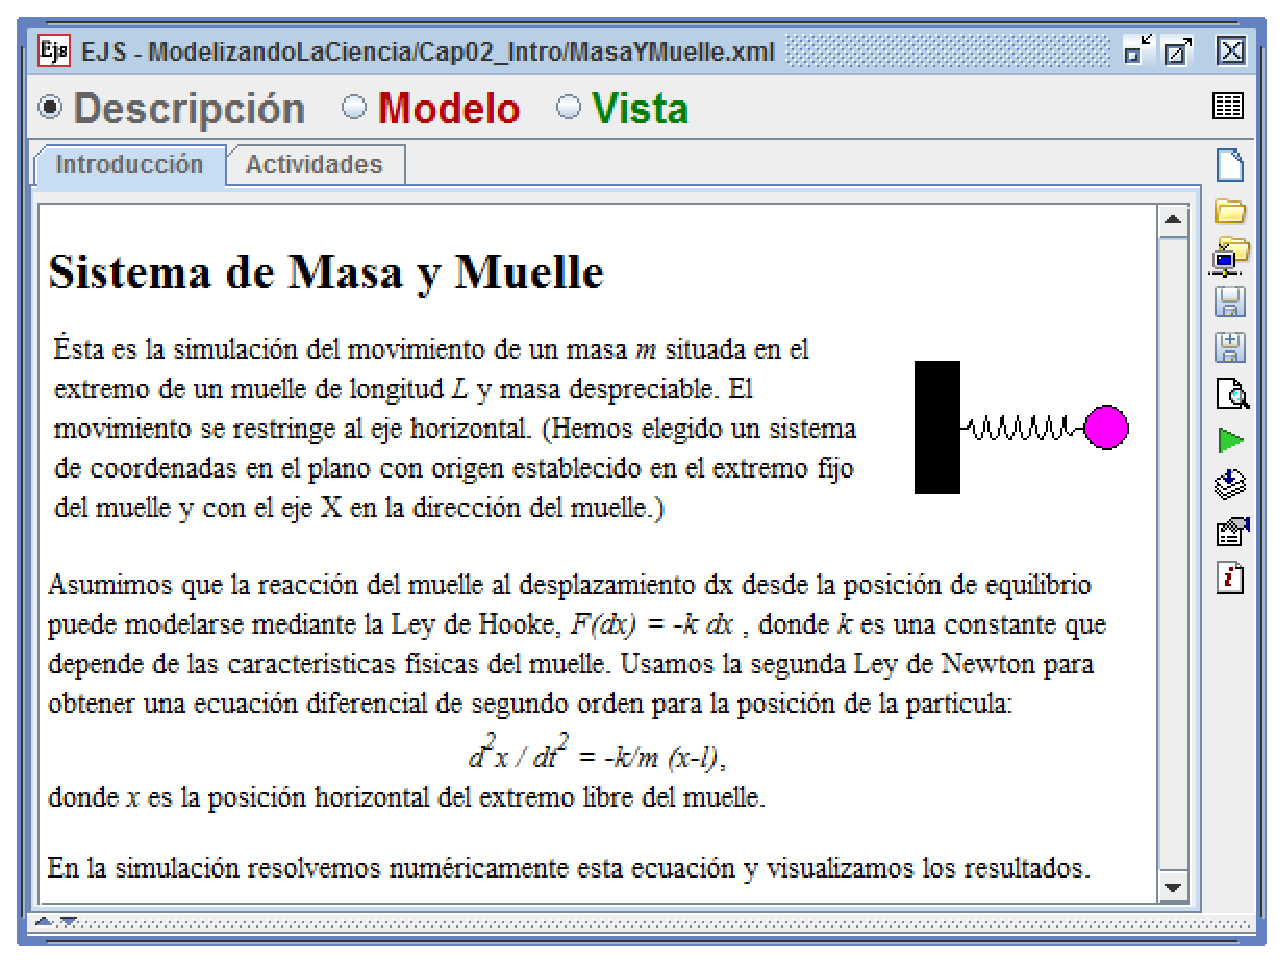
\includegraphics[scale=\scale]{02EjsIntro/images/SpringDesc.eps}
  \caption{The description pages for the mass and spring simulation. Click on a tab to display the page. Right-click on a tab to edit the page.}
  \label{fig:02EjsIntro/SpringDesc}
\end{figure}

A \lit{Description} is HTML\index{HTML} multimedia text that provides information and instructions about the
simulation. HTML stands for HyperText Markup Language and is the Web page format most commonly used on the
Internet.  \ejs\ provides a simple HTML editor that lets you create and modify pages from within \ejs.  You can also
import HTML pages into \ejs\ by right clicking on a tab in the \lit{Description} workpanel. (See
Subsection~\ref{section:02ModifyingDescription}.) Description pages are an essential part of the modeling process and
these pages are distributed with the compiled model when the model is included in a \emph{Launcher} package
or posted on a Web server as an applet. These distribution options are described in
Section~\ref{section:02Distribution}.

\subsection{The \lit{Model} workpanel}\label{section:02Model}

The \lit{Model} workpanel is where the model is made explicit so that it can be implemented by \ejs\ in Java. In this
simulation, we study the motion of a particle of mass $m$ attached to one end of a massless spring of equilibrium
length $l$. The spring is fixed to the wall at its other end and is restricted to move in the horizontal direction.
Although the oscillating mass has a well known analytic solution, it is useful to start with this simple harmonic
oscillator problem so that our output can be compared with an exact analytic result.\index{Simple Harmonic
Motion}

Our model assumes moderate oscillations so that the spring reacts to any given (horizontal) displacement $\delta x$
from the equilibrium with a force given by Hooke's Law,\index{Hooke's Law} $F(\delta x) = - k \delta x$, where $k$ is
the elastic constant of the spring which depends on its physical characteristics. Using Newton's Second
Law\index{Newton's Second Law} we obtain a second-order differential equation for the position of the particle:
\begin{equation}
  \frac{d^2\ x}{dt^2} = -\frac{k}{m}\,(x-l). \label{eq:02EjsIntro/SpringBasic}
\end{equation}
\noindent Notice that we use a system of coordinates with its X-axis along the spring and with its origin at the
spring's fixed end. We simulate this system by solving its differential equation numerically to study how the state
 of the system evolves in time.

Let's examine how we implement the mass and spring model by selecting the \lit{Model} radio button and examining each of
the five panels.

\subsubsection{Declaration of variables}
\begin{figure}[htb]
    \centering
  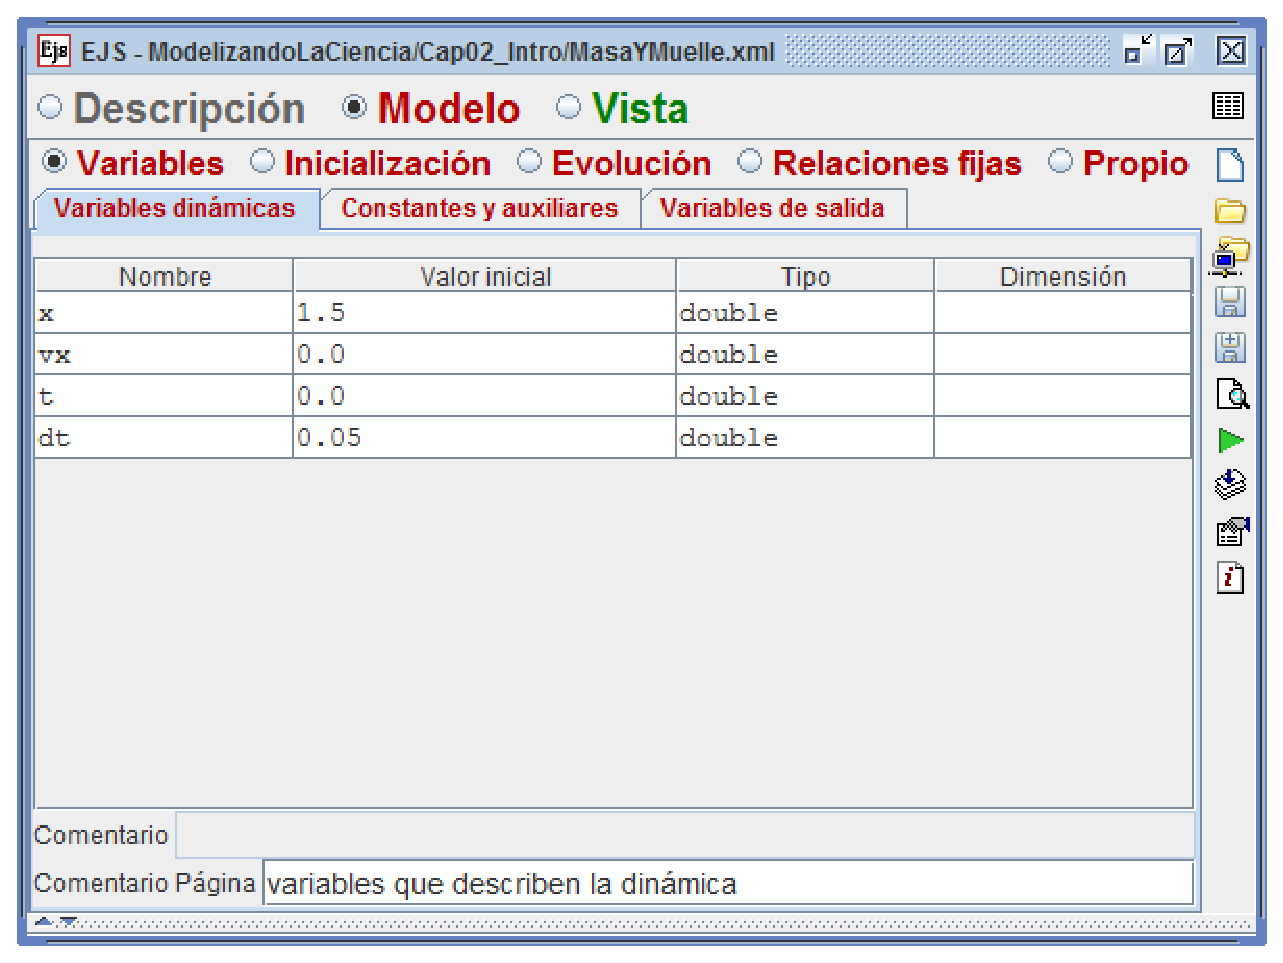
\includegraphics[scale=\scale]{02EjsIntro/images/ModelVariables.eps}
    \caption{The \lit{Model} workpanel contains five subpanels. The subpanel for the definition of mass and spring variables is displayed.}
    \label{fig:02EjsIntro/ModelVariables}
\end{figure}

When implementing a model a good first step is to identify, define, and initialize the variables that describe the
system. The term \emph{variables} is very general and programmers refer to anything that can be given a name, even a
physical constant or a graph, as a variable\index{Model!Variables}. Figure~\ref{fig:02EjsIntro/ModelVariables} shows an
\ejs\ variable table. Each row defines a variable of the model by specifying the name of the variable, its type, its dimension, and
an its initial value.

Variables in computer programs can be of several types depending on the data they hold. Although there are a variety of
data types in Java, the most frequently used are \code{boolean} for true/false values, \code{int} for integer
numbers, \code{double} for double-precision floating point values, and \code{String} for text. A final generic type
called \code{Object} refers to a compound structure such as a three-dimensional body or a graph and opens the world of object-oriented programming.
We use all these variable types in this book, but the mass and spring model uses only variables of type \code{double}.
These numeric variables can be parameters, \index{Model!Parameters} state variables,\index{Model!State variables} or
inputs and outputs of the model.\index{Model!Input and Output}

The \lit{Dimension} column in the table allows us to declare vectors and matrices. The technical term for dimensioned
variables is \emph{arrays}. Arrays can have one or more dimensions and each dimension is specified by the number of
elements in this dimension surrounded by square brackets. Our model does not require arrays, though, so we leave this
column empty. Chapter~\ref{Chapter:Systems} deals with arrays in detail.

The table shown in Figure~\ref{fig:02EjsIntro/ModelVariables} defines the variables used within our model.  We have
declared a variable for the time, \code{t}, for the Y-position of the particle, \code{y}, and for its velocity in the
X-direction, \code{vx}, as well as variables such as the kinetic, potential, and total energies, \code{T}, \code{V},
and \code{E} that don't appear in \eqref{eq:02EjsIntro/SpringBasic}. The reason for these auxiliary variables is made
clear in what follows. The bottom part of the variables panel contains comment fields that we use to provide a
description of the role of each variable in the model. Clicking on a variable displays the corresponding comment.

\subsubsection{The \lit{Initialization} panel}

Correctly setting initial conditions is important when implementing a model because the model must start in a
physically realizable state. Our model is relatively simple and we initialize it by entering values (or simple Java
expressions) in the \lit{Value} column of the table of variables. \ejs\ uses these values when it starts the
simulation.

Advanced models may require an initialization algorithm. For example, a molecular dynamics model may set particle
velocities for an ensemble of particles. The \lit{Initialization} panel allows us to define one or more pages of Java
code that perform the required computation. \ejs\ converts this code into a Java
method\index{Java!method}~\footnote{A Java method is similar to a function or a subroutine in procedural computer languages.}
and calls this method at start-up and whenever the simulation is reset. The mass and spring \lit{Initialization} panel is not
shown here because it is empty. See Subsection~\ref{section:02InspectingConstraints} for an example of how
pages of Java code look like in Ejs.



\subsubsection{The evolution of the model}

The goal of our simulation is to study how the mass and spring system evolves in time and the \lit{Evolution} panel
performs this task.  \ejs\ allows us to program our own algorithm and we use this option when studying
numerical differential equation algorithms or stochastic (probabilistic) algorithms. Although we can always program our
own evolution algorithm, the \lit{Evolution} panel has a second option that allows us to enter ordinary differential
equations (ODEs), such as \eqref{eq:02EjsIntro/SpringBasic}, without programming.

\ejs\ provides a dedicated editor that lets us specify differential equations in a format that resembles mathematical
notation and automatically generates the correct Java code. Although the mass and spring model
can be solved with a simple ODE algorithm, our numerical methods library contains very sophisticated algorithms and \ejs\ can apply these algorithms to large systems of vector differential equations with or without discontinuous events (events are discussed in Chapter~\ref{chapter:Events}).

Let's see how the differential equation editor works for the mass and spring model. Because ODE algorithms solve
systems of first-order ordinary differential equations, a higher-order equation, such as
\eqref{eq:02EjsIntro/SpringBasic}, must be recast into a first-order system.   This is easily done by treating the
velocity as an independent variable that obeys its own equation:
\begin{eqnarray}
  \frac{d\ x} {dt} &=& v_x                  \label{eq:02EjsIntro/SpringBasicODE1} \\
  \frac{d\ v_x}{dt} &=& -\frac{k}{m}\,(x-l). \label{eq:02EjsIntro/SpringBasicODE2}
\end{eqnarray}
\noindent This explains why we declared the \code{vx} variable in our table of variables.

Clicking on the \lit{Evolution} panel displays the ODE editor shown in
Figure~\ref{fig:02EjsIntro/ModelEvolution}.
\begin{figure}[htb]
    \centering
  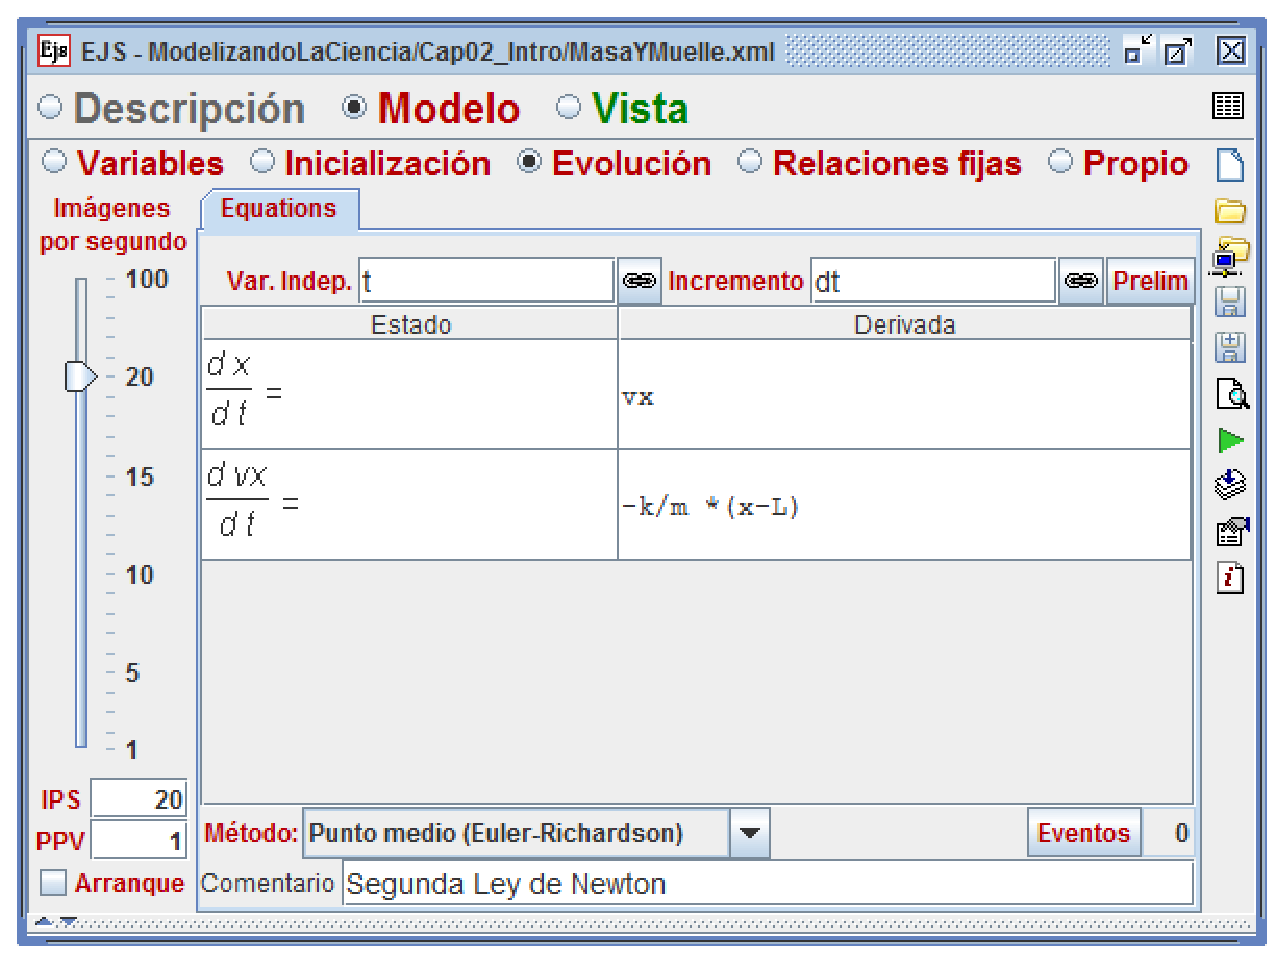
\includegraphics[scale=\scale]{02EjsIntro/images/ModelEvolution.eps}
    \caption{The ODE evolution panel showing the mass and spring differential equation and the numerical algorithm selected.}
    \label{fig:02EjsIntro/ModelEvolution}
\end{figure}
Notice that the ODE editor displays \eqref{eq:02EjsIntro/SpringBasicODE1} and \eqref{eq:02EjsIntro/SpringBasicODE2}
using Java syntax to specify multiplication with the \lit{*} character. Fields near the top of the editor specify the
independent variable \code{t} and the variable increment \code{dt}.  Numerical algorithms approximate the exact ODE solution by advancing the state in discrete steps and the increment determines this step size. A dropdown menu at the bottom of the editor lets us select the ODE solver (numerical algorithm) that advances the solution from the current value of time, \code{t}, to the next value, \code{t+dt}. The events field at the bottom of the panel tells us that we have
not defined any events for this differential equation.

The left-hand side of the evolution panel includes fields that determine how smooth and how fast the simulation runs.
The \lit{Frames per second} (\lit{FPS}) option, which can be selected using either a slider or an input field, specifies how many times per second we want our simulation to repaint the screen. The \lit{Steps per display} (\lit{SPD}) input field
specifies how many times we want to advance (step) the model before repainting. The current value of \code{20} frames per second produces a smooth animation that, together with the prescribed value of one step per display and \code{0.05} for
\code{dt}, results in a simulation which runs (approximately) at real time. We will almost always use the default
setting of one step per display. However, there are situations where the model's graphical output consumes a
significant amount of processing power and where we want to speed the numerical work. In this case, we can increase the
steps per display parameter so that the evolution algorithm is performed multiple times before the visualization is redrawn.
Finally, the \lit{Autoplay} check box indicates whether the simulation should start when the program begins. This box
is unchecked so that we can change the initial conditions before starting the evolution.

The \lit{Evolution} panel handles the technical aspects of the mass and spring ODE model without Java programming.  The
simulation advances the state of the system by numerically solving the model's differential equations using the
Midpoint algorithm selected. The algorithm steps from the current state at time \code{t} to a new state at a new time
\code{t+dt} before the visualization is redrawn. The simulation repeats this evolution step \code{20} times per second
on computers with modest processing power. The simulation may run slower and not as smooth on computers with
insufficient processing power or if the computer is otherwise engaged, but it should not fail.

\subsubsection{Constraints among variables}\label{section:02InspectingConstraints}

Not all variables within a model are computed using the evolution algorithm. Some may be computed from other variables
using a simple formula. In this book, we refer to variables that are computed using the evolution algorithm as state variables or
dynamical variables and we refer to variables that depend on these variables as auxiliary or output variables. In the mass and
spring model the kinetic, potential, and total energies of the system are output variables because they are computed
from state variables using:
\begin{eqnarray}
  T &=& \frac{1}{2} m {v_x}^2              \label{eq:02EjsIntro/SpringEnergy1} \\
  V &=& \frac{1}{2} k (x-l)^2    \label{eq:02EjsIntro/SpringEnergy2} \\
  E &=& T + V  \;.                            \label{eq:02EjsIntro/SpringEnergy3}
\end{eqnarray}
We refer to this situation by saying that there exist fixed \emph{constraints} among the
model's variables.~\footnote{To avoid misunderstandings, lets us explicitly state that our use of the word
\emph{constraints} is \textbf{not} directly related to the concept of constraints in Classical Mechanics.}

The \lit{Constraints} panel shown in Figure~\ref{fig:02EjsIntro/ModelConstraints} is used to write constraints among
variables. Notice how easy it is to translate \eqref{eq:02EjsIntro/SpringEnergy1} through
\eqref{eq:02EjsIntro/SpringEnergy3} into Java code. The most difficult thing to remember is (again) to
use the multiplication character \lit{*} and to place a semicolon at the end of every Java statement.

\begin{figure}[htb]
    \centering
  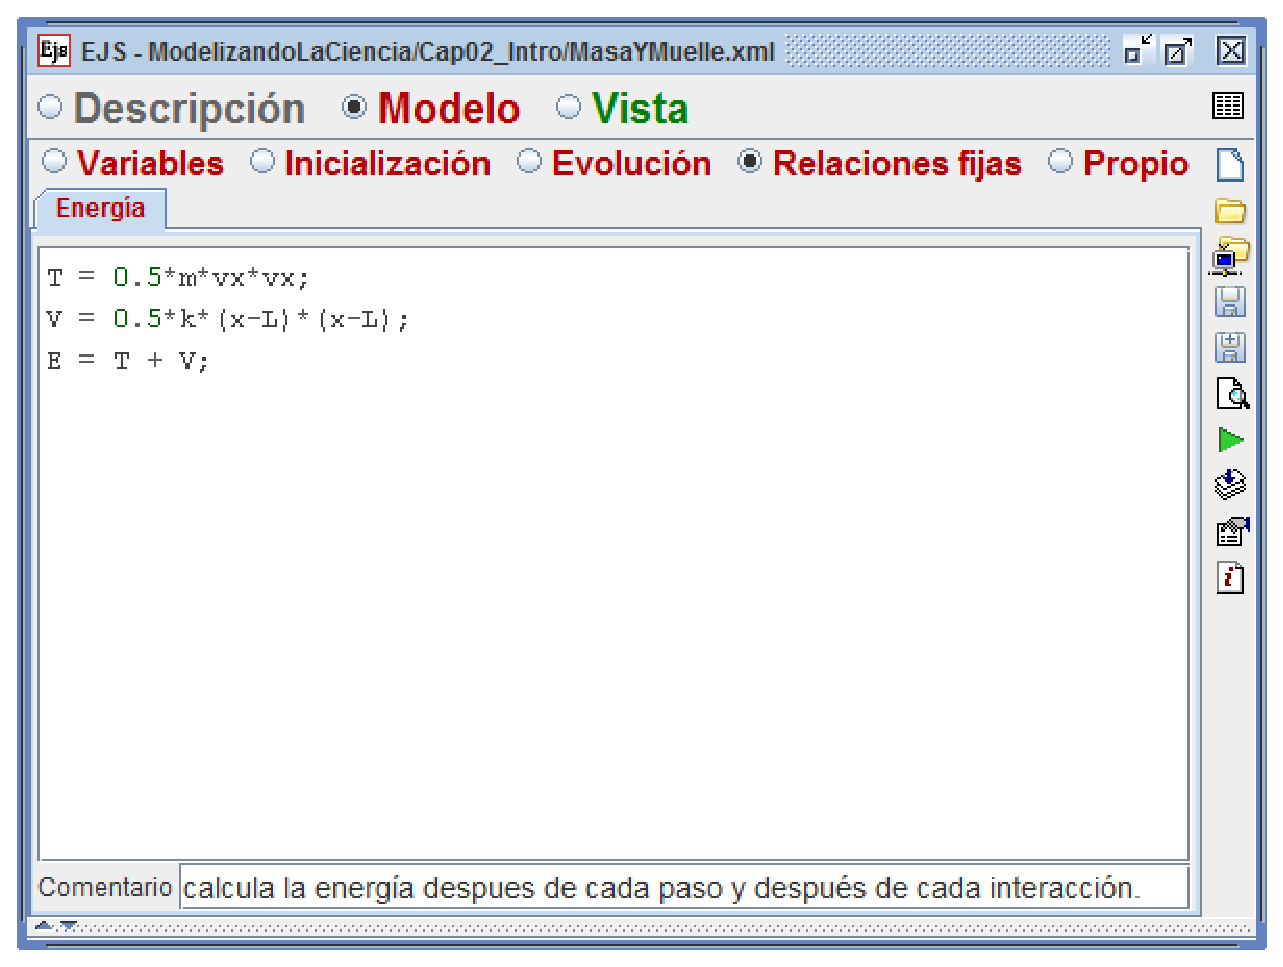
\includegraphics[scale=\scale]{02EjsIntro/images/ModelConstraints.eps}
    \caption{The constraints for the mass and spring model.}
    \label{fig:02EjsIntro/ModelConstraints}
\end{figure}

You may wonder why we do not write constraint expressions by adding a code page after the ODE page in the
\lit{Evolution} panel. After all, evolution pages execute sequentially and this would correctly update the output variables after every
step. The reason that the \lit{Evolution} panel should not be used is that constraint equations must \emph{always} hold
and there are other ways, such as mouse actions, that affect state variables. \ejs\ automatically evaluates constraints
after initialization, after every evolution step, and whenever there is \emph{any} user interaction with the simulation
interface. For this reason, it is important that fixed relationships among variables be written in the
\lit{Constraints} panel.

\subsubsection{Custom pages}

Finally, there is a fifth panel in the \lit{Model} workpanel labeled \lit{Custom}.  This panel can be used to define Java methods that can be used throughout the model.  This panel is empty because our model currently doesn't require additional methods, but we make use of this panel when we modify our mass and spring example in Section~\ref{section:02Modifying}.  We should mention that a custom method is not used unless it is explicitly invoked from another panel.

% ---------------------------------------------
\subsection{The \lit{View} workpanel}
% ---------------------------------------------

The third \Ejs\ workpanel is the \lit{View}.  This workpanel allows us to create a graphical interface that includes visualization, user interaction, and program control with a minimum amount of programming.  Figure~\ref{fig:02EjsIntro/SpringInterface} shows the view for the mass and spring model. Select the \lit{View} radio button to examine how this view is created.

The right frame of the view workpanel of \ejs, shown in Figure~\ref{fig:02EjsIntro/View}, contains a collection of \emph{view elements},\index{Ejs!view elements} grouped by functionality. View elements are building blocks that can be combined to form a complete user interface and each view element is a specialized object with an on-screen representation. To display information about a given element, click on its icon
and press the \lit{F1} key. To create a user interface, we create a frame (window) and add elements, such as buttons and graphs, using ``drag and drop'' as described in Section~\ref{section:02Modifying}.
\begin{figure}[htb]
    \centering
  \includegraphics[scale=\scale]{02EjsIntro/images/View.eps}
    \caption{The \lit{View} workpanel showing the \emph{Tree of Elements} for the mass and spring user interface. }
    \label{fig:02EjsIntro/View}
\end{figure}

The \emph{Tree of Elements} shown on the left side of Figure~\ref{fig:02EjsIntro/View} displays the structure of the mass and spring user interface. Notice that the simulation has two windows, a Java \code{Frame} and a Java \code{Dialog}.  The tree displays descriptive names and icons for these and other elements.  The \emph{panels} are \emph{containers} whose primary purpose is to visually group (organize) elements within the user interface. Right-click on an element of the tree to get a menu that helps change this structure.

Each view element has a set of internal parameters, called \emph{properties},\index{Ejs!view element properties} which configure the element's appearance and behavior. We edit these properties by double clicking on the element in the tree to display a table known as a properties inspector.  Visual properties, such as color, are often set to a constant value, such as \code{RED}. We can also use a variable from the model to set an element's property. This ability to bind a property to a variable without programming is the key to turning our view into a dynamic and interactive visualization.

Let's see how this works in practice. Double-click on the \code{massParticle} element in the tree to display the element's properties inspector. This element is, of course, the mass that is attached at the free end of the spring. The mass' table of properties appears as shown in Figure~\ref{fig:02EjsIntro/SpringBallProperties}.
\begin{figure}[htb]
    \centering
  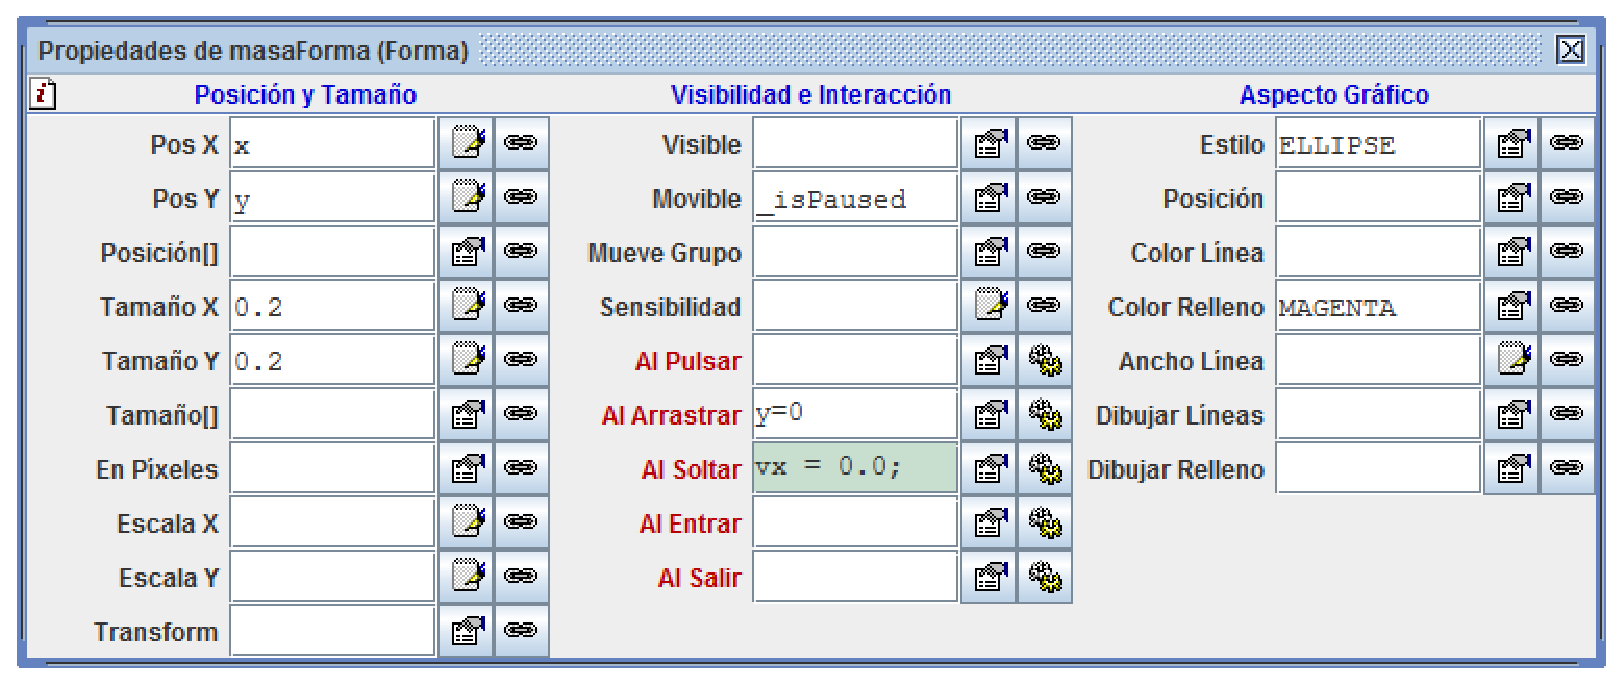
\includegraphics[scale=\scale]{02EjsIntro/images/SpringBallProperties.eps}
    \caption{The table of properties of the \code{ballParticle} view element. }
    \label{fig:02EjsIntro/SpringBallProperties}
\end{figure}

Notice the properties that are given constant values. The \code{Style}, \code{Size X}, \code{Size Y}, and \code{Fill Color} properties produce an ellipse of size \code{(0.2,0.2)} units (which makes a circle) filled with a magenta color. More importantly, the \code{X} and \code{Y} properties of  the particle are bound to the \code{x} and \code{y} variables of the model. This simple assignment establishes a bidirectional connection between model and view. These variables change as the model evolves and the particle follows the \code{x} and \code{y} values. If the user drags the particle to a new location, the \code{x} and \code{y} variables in the model change accordingly.

Elements can also have \emph{action properties}\index{Ejs!action properties} which can be associated with Java code. (To help distinguish them, action properties have their labels displayed in red.) User actions, such as dragging or clicking, invoke their corresponding action property, thus providing a simple way to control the simulation. In our example, when the user presses with the mouse on the particle, the simulation is paused as indicated by the built-in method \code{\_pause()}. Then, as the user drags the particle, the code on the \code{On Drag} property repeatedly sets the \code{y} variable to \code{0}. This restricts the motion of the particle to the horizontal direction. Finally, when the mouse button is released, the following code is executed:

\begin{listing}
\begin{verbatim}
vx = 0.0;            // sets the velocity to zero
_view.resetTraces(); // clears all plots
\end{verbatim}
\end{listing}

\note{Because this code spans more than one line, the \code{On Release} property field shows a darker (sort of green) background color. Clicking on the  first icon next to the field displays a small window showing the code fragment. Other data types, such as boolean properties, have different editors.  The second inspector icon provides a listing of variables or methods that can be used to set the property value.}

The particle illustrates the different types of properties and their possible values. Feel free to explore the properties of other elements of the view.  For instance, the \code{displacementTrace} and \code{velocityTrace} elements correspond to the displacement and velocity time plots in the second window of our view, respectively.

\subsection{The completed simulation}
\Ejs\ provides a simple yet powerful conceptual structure to create simulations with minimal programming. We express
our knowledge of the model within workpanels and \ejs\ combines this information to create a program.

When modeling the mass and spring, we first created a table of variables that describes our model and initialized these
variables using a column in the table. We then used an evolution panel with a high-level editor for systems of
first-order ordinary differential equations to specify how the state variables advance in time. Finally, we wrote
constraints to compute auxiliary or output variables that can be expressed using expressions involving state variables.

The program's graphical user interface and high-level visualizations were created by dragging objects from the
\lit{Elements} pallet into the \lit{Tree of Elements}. Element properties were set using a properties editor and some were associated with variables from the model.

When the program is compiled as described in Section~\ref{section:02Running}, the table of variables is used to reserve memory and each variable is initialized. The program then executes the constraints pages to insure that all dependent (output) variables have the correct value. This brings the model into a consistent state.

The evolution starts when the play button in the programs' user interface is pressed. The program executes a numerical method to advance our differential equation by $0.05$ time units and again executes our constraints code.  Data is then passed to view elements, such as graphs, and these elements are repainted. This process is repeated $20$ times per second.

% -----------------------------------------------------
\section{Running the Simulation}\label{section:02Running}
% -----------------------------------------------------

It is time to run the simulation. Click on the \lit{Run} icon of \ejs' taskbar, \includegraphics[scale=\linescale]{images/run.eps}, to processes the information in the workpanels.  \Ejs\ generates the Java code and compiles it, collects auxiliary and library files, and runs the simulation. All at a single mouse click.

When running a simulation, \ejs\ changes its \lit{Run} icon to red and prints informational messages saying that the simulation has been successfully generated and that it is running. Notice that the two ``Ejs windows'' disappear and are replaced by new (but similar) windows without the ``Ejs windows'' suffix in their titles.  These views respond to user actions. Click and drag the particle to a desired initial horizontal position and then click on the \lit{Play} button. The particle oscillates about is equilibrium point and the plot displays displacement and velocity data as shown in Figure~\ref{fig:02EjsIntro/SpringRunning}.

\begin{figure}[htb]
  \centering
  \subfigure{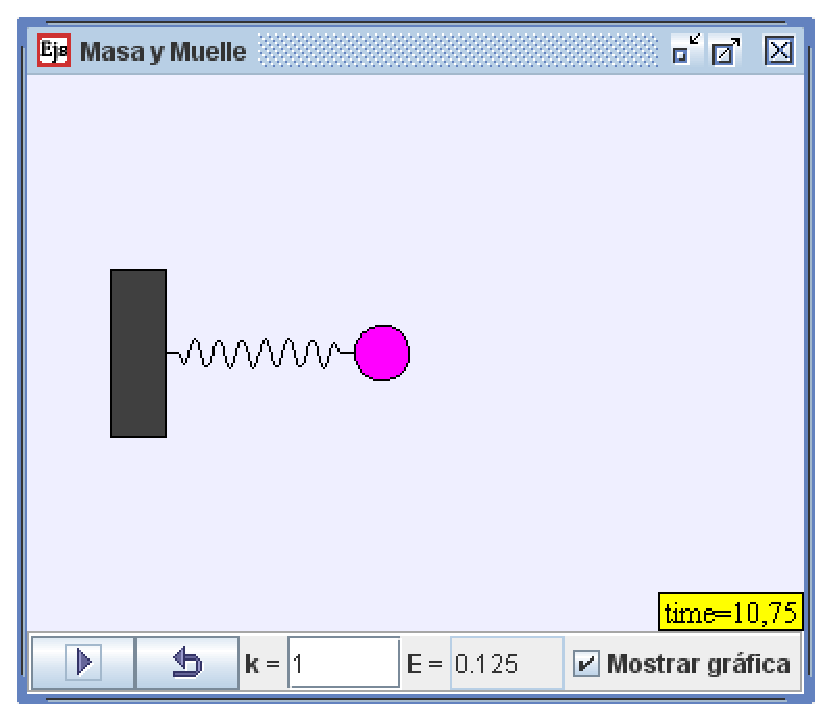
\includegraphics[scale=\scale]{02EjsIntro/images/SpringRunning1.eps}}
  \subfigure{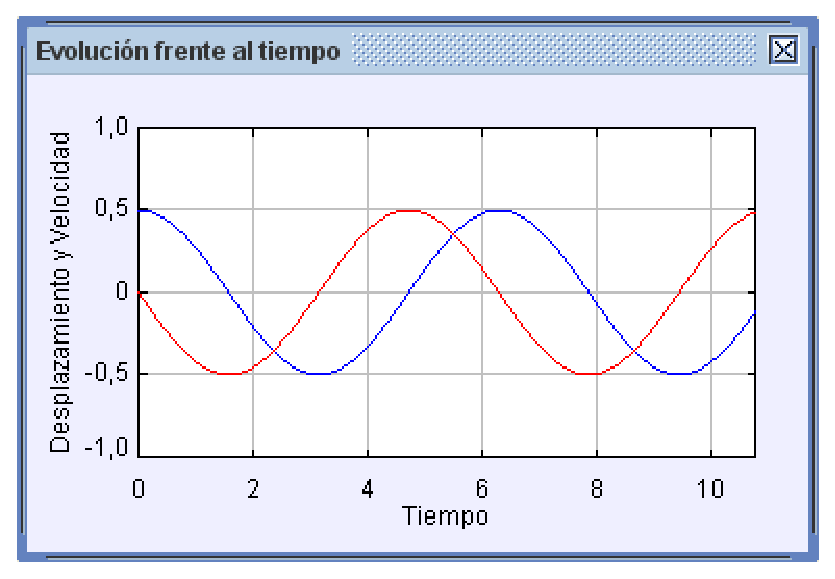
\includegraphics[scale=\scale]{02EjsIntro/images/SpringRunning2.eps}}
  \caption{The mass and spring simulation displays an interactive representation of the model and a graph with displacement and velocity data.}
  \label{fig:02EjsIntro/SpringRunning}
\end{figure}

The simulation is now ready for distribution.
To exit the program, close the simulation main (left) window.

\subsection{Distribution of simulations}\label{section:02Distribution}\index{Distribution of simulations}

Simulations created with \ejs\ are stand alone Java programs that do not depend on \ejs\ and can be distributed without \ejs\ for other people to use. There are many ways of doing this.

When a simulation is run, \ejs\ creates a Java program in a subdirectory within the \file{\_apps} subdirectory within the \file{Simulations} directory. Look for a subdirectory called  \file{\_apps/\_ModelingScience\-/02EjsIntro/Mass\-And\-Spring.app}. This subdirectory contains the files required to run the simulation. Double-click on the \file{massAndSpring.jar} file to run our example. In order to keep this jar file small, it contains only the compiled code specific to our simulation.  The jar file requires resources that are located in the \file{\_library} directory four levels up in the \file{Simulations} directory.  You can, in principle, distribute both the \file{\_apps} and the \file{\_library} directories, together with instructions to navigate down to the \file{MassAndSpring.app} directory.  This distribution mechanism is efficient when distributing multiple simulations because the \ejs\ library is used by every simulation.

Because distributing multiple files is inconvenient and error prone, \ejs\ can package a simulation in a single executable jar file. Right-click (left-clicking is discussed below) on the \lit{Package} icon, 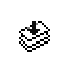
\includegraphics[scale=\linescale]{images/package.eps}, on the \ejs' taskbar to display a popup menu and select the \lit{Package current simulation only} entry. A file browser appears that lets you choose a name for the self-contained jar package. Although the jar file that is created is much larger than the simulation-only file, it contains the complete library and is ready to be distributed separately on CD or via the Internet.

Packaging and distributing multiple stand-alone jar files each of which contains the library is a waste of resources if multiple simulations are used in a curriculum module.  A more efficient and elegant distribution mechanism is to package multiple simulations and their associated curricular material in a single jar file. We refer to such a jar as  a \emph{Launcher}\index{Launcher packages} package and it is easy to create such a package by left-clicking on the taskbar's \lit{Package} icon.

\begin{figure}[htb]
    \centering
  \includegraphics[scale=\scale]{02EjsIntro/images/Launcher.eps}
    \caption{Multiple simulations can be distributed in a Launcher package. [NOTE: Replace image when additional simulations are ready for distribution.]}
    \label{fig:02EjsIntro/Launcher}
\end{figure}

Executing a Launcher package provides easy access to multiple simulations as shown in Figure~\ref{fig:02EjsIntro/Launcher}.  Clicking on a launch node (green arrow) in the table of contents tree displays the simulation's description pages and double clicking the node runs the simulation.  All models described in this book are ready-to-use in the \file{ejs\_modeling\_science.jar} package on the CD that accompanies this book.  A more complete discussion of Launcher packages is available in Appendix~\ref{chapter:ADistribution}.

A Java applet is a program that is embedded in a web page and distributed over the Internet from a web server and \Ejs\ supports this distribution mechanism as well. Open the \file{MassAndSpring.html} file in the \file{MassAndSpring.app} subdirectory with your favorite web browser and you will see the mass and spring model as shown in Figure~\ref{fig:02EjsIntro/SpringHTML}.

\begin{figure}[htb]
    \centering
  \includegraphics[scale=\scale]{02EjsIntro/images/SpringHTML.eps}
    \caption{The main HTML page for our simulation. }
    \label{fig:02EjsIntro/SpringHTML}
\end{figure}

\ejs\ creates an HTML page that contains the applet and publishes this page along with the model's description pages in an HTML frameset with a table of contents. Click on the \lit{Simulation} entry in the table of contents to run the Java applet\index{Java applet} as shown in Figure~\ref{fig:02EjsIntro/SpringHTML_simulation}.~\footnote{Your browser must have a Java plug-in installed for the applet to run. Depending on your security settings, you may also need to explicitly allow active content, such as applets, to appear.}

\begin{figure}[htb]
    \centering
  \includegraphics[scale=\scale]{02EjsIntro/images/SpringHTML_simulation.eps}
    \caption{The simulation running as a Java applet. }
    \label{fig:02EjsIntro/SpringHTML_simulation}
\end{figure}

Publishing \ejs\ applets on a Web server is now straightforward. Just copy the \file{\_apps} and the \file{\_library} directories into the same directory of your Web server. Because HTML files in the \file{MassAndSpring.app} subdirectory refer to the \file{\_library} directory in its current location, you must edit references within your HTML pages if you change the relative location of your files.

An \ejs\ XML file contains a complete blueprint for a simulation and an easy way for \ejs\ users to share their simulations is to distribute the simulation's XML file together with auxiliary files, such as images. (Auxiliary files are listed within the simulation's information panel that appears when you click on the top-right icon 
\includegraphics[scale=\linescale]{images/properties.eps} of the interface of \ejs.)  The \file{MassAndSpring.xml} file and auxiliary files are in the \file{\_ModelingScience} directory and are less than $20$ KByte whereas a compiled stand-alone \file{massAndSpring.jar} file is $2$ MByte.  An efficient procedure is to gather a model's files into a ``zip'' archive and send them to other \ejs\ users who ``unzip'' them in their own \file{Simulations} directory.

To make the \ejs\ modeling cycle even easier, simulations packaged by \ejs\ within a jar file include a copy of all XML and resource files. Hence, if a user runs an \ejs\ simulation from a jar file (either a single simulation or a Launcher package as described above), right-clicking on any graphics panel within the simulation displays a popup menu which contains an option to go from the running program to \ejs. (\ejs\ must, of course, be installed.) This will extract the XML and all required auxiliary files from the jar file, search for the \ejs\ installation in the user's hard disk, copy the files into the correct location, and run \ejs\ with this simulation loaded. The user can then inspect, run, and modify the simulation exactly as we are doing in this chapter. \note{Users running a Java applet cannot access \ejs\ on the local hard disk because of security restrictions imposed by browsers. However, an advanced procedure known as \emph{signing the applet}\index{Signing applets} overcomes this limitation. To learn how to sign a Java applet, visit http://developers.sun.com and search for ``Signing applets''.}

\ejs\ is designed to be both an authoring and a modeling tool and we suggest that you now experiment with it to learn how you can create and distribute your own models. As a start, we recommend that you run the mass and spring simulation and go through the activities in the second page of the \lit{Description} panel.  We modify this simulation in the next section.
% -----------------------------------------------------
\section{Modifying the Simulation}\label{section:02Modifying}
% -----------------------------------------------------

As we have seen, a prominent and distinctive feature of \Ejs\ is that it allows us to create and study a simulation at a high science-oriented level of abstraction. We inspected an existing mass and spring model and its user interface in the previous section. We now illustrate additional capabilities of \Ejs\ by adding friction and a driving force and by adding a visualization of the system's phase space.

\subsection{Extending the model}\label{section:02ModifyingModel}

We add damping in our model by introducing a viscous (Stoke's Law) force that is proportional to the negative of the velocity $F_f = - b\,v_x$ where $b$ is the coefficient of dynamic friction. We also add an external time-dependent driving force which takes the form of a sinusoidal function $F_e(t)=A\,\sin(\omega\, t)$. The introduction of these two forces changes the second-order differential equation \eqref{eq:02EjsIntro/SpringBasic} to:
\begin{equation}
  \frac{d^2\ x}{dt^2} = -\frac{k}{m}\,(x-l) - \frac{b}{m}\,\frac{d\ x}{dt} + \frac{1}{m}\,f_e(t), \label{eq:02EjsIntro/SpringComplete}
\end{equation}
\noindent or, to the equivalent of equations \eqref{eq:02EjsIntro/SpringBasicODE1} and \eqref{eq:02EjsIntro/SpringBasicODE2}:
\begin{eqnarray}
  \frac{d\ x} {dt} &=& v_x                  \label{eq:02EjsIntro/SpringCompleteODE1} \\
  \frac{d\ v_x}{dt} &=& -\frac{k}{m}\,(x-l) - \frac{b}{m}\,v_x + \frac{1}{m}\,f_e(t). \label{eq:02EjsIntro/SpringCompleteODE2}
\end{eqnarray}

\subsubsection{Adding variables}

The introduction of new force terms requires that we add variables for the coefficient of dynamic friction and for the amplitude and frequency of the sinusoidal driving force.  Return to the \lit{Model} workpanel of \ejs\ and select its \lit{Variables} panel. Right-click on the tab of the existing page of variables to bring in its popup menu, as in Figure~\ref{fig:02EjsIntro/ModifyVariables1}.
Select the \lit{Add a new page} entry as shown in this same figure. Enter \code{Damping and driving forces} for the new table name in the dialog and an empty table will appear.

\begin{figure}[htb]
    \centering
  \includegraphics[scale=\scale]{02EjsIntro/images/ModifyVariables1.eps}
    \caption{The popup menu for a page of variables. }
    \label{fig:02EjsIntro/ModifyVariables1}
\end{figure}

We now use the new table to declare the needed variables. We could have used the already existing table but declaring multiple pages helps us organize the variables by category. Double-click on a table cell to make it editable and navigate through the table using the arrows or tab keys. Type \code{b} in the \lit{Name} cell of the first row, and enter the value \code{0.1} in the \lit{Value} cell to its right. This is all we need to do because the \code{double} type selected is already correct. Notice that when you fill in a variable name, a new row appears automatically. Proceed similarly to declare a new variable for the driving force's \code{amplitude} with value \code{0.2} and for its \code{frequency} with value \code{2.0}. You should document the meaning of these variables by typing a short comment for each at the bottom of the table. Our final table of variables is shown in Figure~\ref{fig:02EjsIntro/ModifyVariables2}.  You can ignore the empty row at the end of the table or remove it by right-clicking on that row and selecting \lit{Remove this variable} from the popup menu that appears.

\begin{figure}[htb]
    \centering
  \includegraphics[scale=\scale]{02EjsIntro/images/ModifyVariables2.eps}
    \caption{The new table of variables for the damping and forcing terms. }
    \label{fig:02EjsIntro/ModifyVariables2}
\end{figure}

\subsubsection{Modifying the evolution}

We now modify the differential equations on our evolution page by adding expressions for the new terms in equation
\eqref{eq:02EjsIntro/SpringCompleteODE2}. Go to the evolution panel, double-click on the \lit{Rate} cell of the
second equation, and edit it to read:

\begin{listing}
\begin{verbatim}
-k/m * (x-l) - b*vx/m + force(t)/m
\end{verbatim}
\end{listing}

Notice that we are using a method (function) named \code{force} that has not yet been defined.
We could have written an explicit expression for our sinusoidal function. However, defining a \code{force} method promotes cleaner and more readable code and allows us to introduce custom methods.

\subsubsection{Adding custom code}

The \code{force} method is defined using the \lit{Custom} panel of the \lit{Model}. Go to this panel and click on the empty central area to create a new page of custom code. Name this page \lit{Driving force}. You will notice that the page is created with a code template that defines a method. Edit this code to read:

\begin{listing}
\begin{verbatim}
public double force (double time) {
  return amplitude * Math.sin(frequency*time); // sinusoidal driving force
}
\end{verbatim}
\end{listing}
\noindent Please type this code exactly as shown including capitalization. Compilers always complain if there is any syntax error.

Notice that we pass the time at which we want to compute the driving force to the method as an input parameter. This is very important. It would be incorrect to ask the method to use the value of the variable \code{t}, as in:

\begin{listing}
\begin{verbatim}
public double force () { // incorrect implementation of the force method
  return amplitude * Math.sin(frequency*t);
}
\end{verbatim}
\end{listing}
\noindent The reason is that most numerical solvers evaluate the \lit{Rate} column at intermediate values of the independent variable $t$ as they evolve the system from $t$ to $t+\Delta t$ during a single step. In order to compute the rate at these intermediate times, the independent variable and any other dynamic variable which is differentiated in the \lit{State} column of the ODE editor must be passed explicitly as a parameter to any method that is called from the \lit{Rate} column. Model variables which remain constant during an evolution step may be used directly in the method's body.

\subsection{Improving the view}\label{section:02ModifyingView}

We now add a phase space (displacement vs. velocity) visualization of the system's evolution to the \lit{View}. We also add new input fields to display and modify the value of the \code{b}, \code{amplitude}, and \code{frequency} parameters.

Go to the \lit{View} workpanel and notice that the \lit{Interface} palette contains many subpanels.  Click on the tab with the 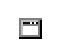
\includegraphics[scale=\linescale]{images/Groups/Containers.eps} icon to display the \lit{Windows, containers, and drawing panels} palette of view elements.  Click on the icon for a plotting panel, 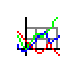
\includegraphics[scale=\linescale]{images/Elements/PlottingPanel.eps}, within this palette. You can rest (hover) the mouse cursor over an icon to display a hint that describes the element if you have difficulty recognizing the icon.  Selecting an element changes the background color on the palette and changes the cursor to a magic wand, 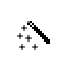
\includegraphics[scale=\linescale]{images/create.eps}. This indicates that \ejs\ is ready to create an element of the selected type.

Click on the \code{dialog} element in the tree (the left frame of the \ejs\ workspace) as shown in Figure~\ref{fig:02EjsIntro/ModifyViewAddPlottingPanel} to add the plotting panel to the view.

\begin{figure}[htb]
    \centering
  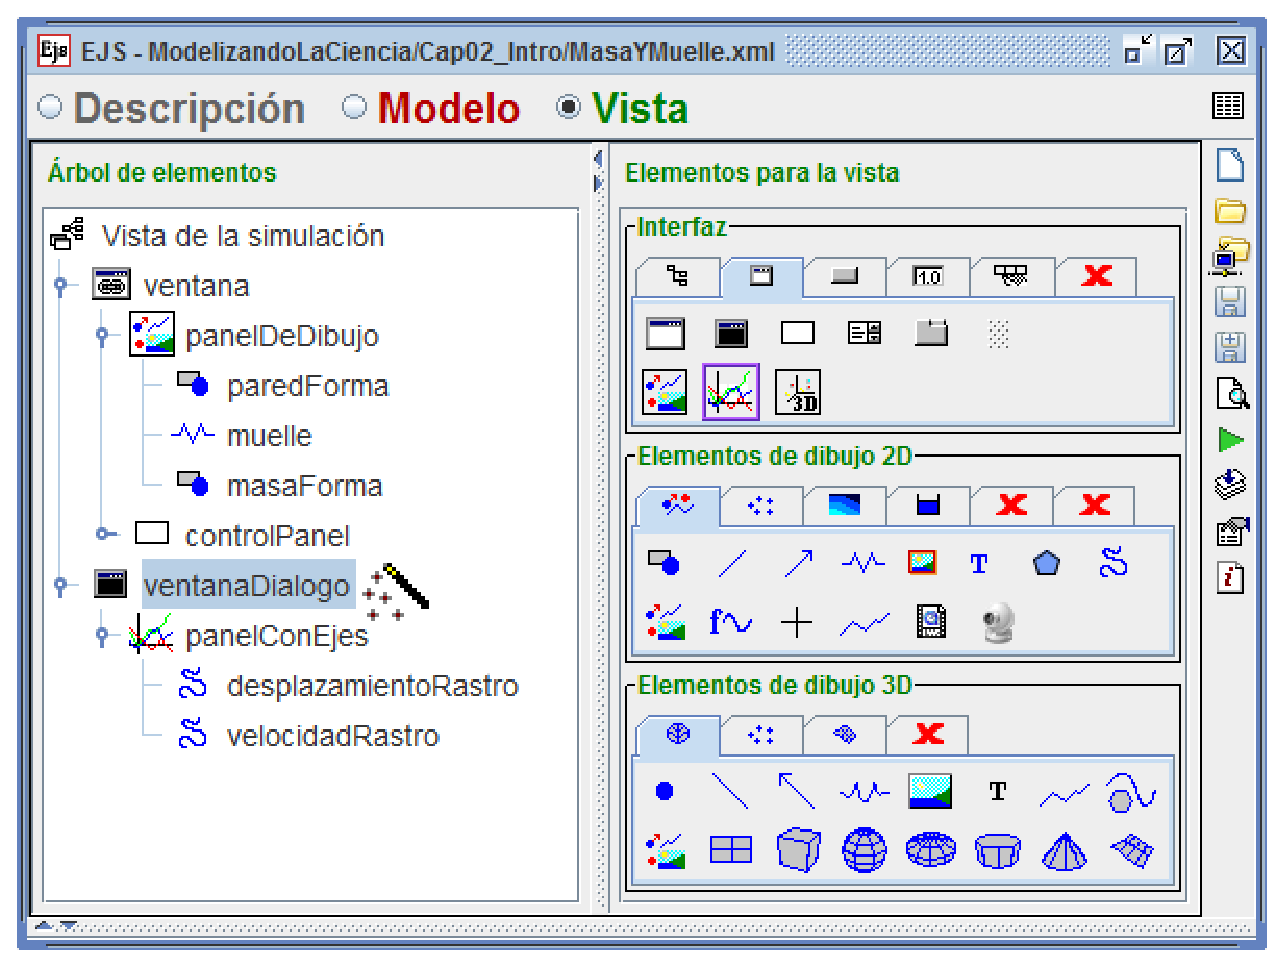
\includegraphics[scale=\scale]{02EjsIntro/images/ModifyViewAddPlottingPanel.eps}
    \caption{Creation of a plotting panel as child of the \code{dialog} element of the view. }
    \label{fig:02EjsIntro/ModifyViewAddPlottingPanel}
\end{figure}

\ejs\ asks for a name for the new element and then creates the element as a child within the existing \code{dialog}. A new plot appears but the dialog is too small.  Return to the design mode (get rid-off the magic wand) by clicking on any blank area within the tree of elements or hitting the \lit{Esc} key. Resize the dialog box by dragging its corner. You can also fix the size problem by double-clicking on the \code{dialog} element in the tree to show its properties table and changing its \code{Size} property to \code{400,400}, thus doubling its height. Finally, edit the properties table of the newly created plotting panel element to set the \code{Title} property to \code{Phase Space}, the \code{Title X} property to \code{Displacement}, and the \code{Title Y} property to \code{Velocity}. Set the minima and maxima for both X and Y scales to \code{-1} and {1}, respectively, and leave the other properties untouched.

The plotting panel is, as its name suggest, the container for our phase-space plot. Phase space data is drawn in this panel using an element of type \code{Trace}, 
\includegraphics[scale=\linescale]{images/Elements/Trace.eps}.  Find the \code{Trace} element in the \code{2D Drawables} palette and follow the same procedure as before.  Select the \code{Trace} element and create an element of this type by clicking with the magic wand on the phase space panel. Finally, edit the properties of the new trace element to set its \code{X} input property to \code{x-l} and its \code{Y} input property to \code{vx}. This assignment causes the simulation to add a new \code{(x-l,vx)} point to the trace after each evolution step, thus drawing the phase-space plot shown in Figure~\ref{fig:02EjsIntro/ModifyRunning}.
\begin{figure}[htb]
  \centering
  \subfigure{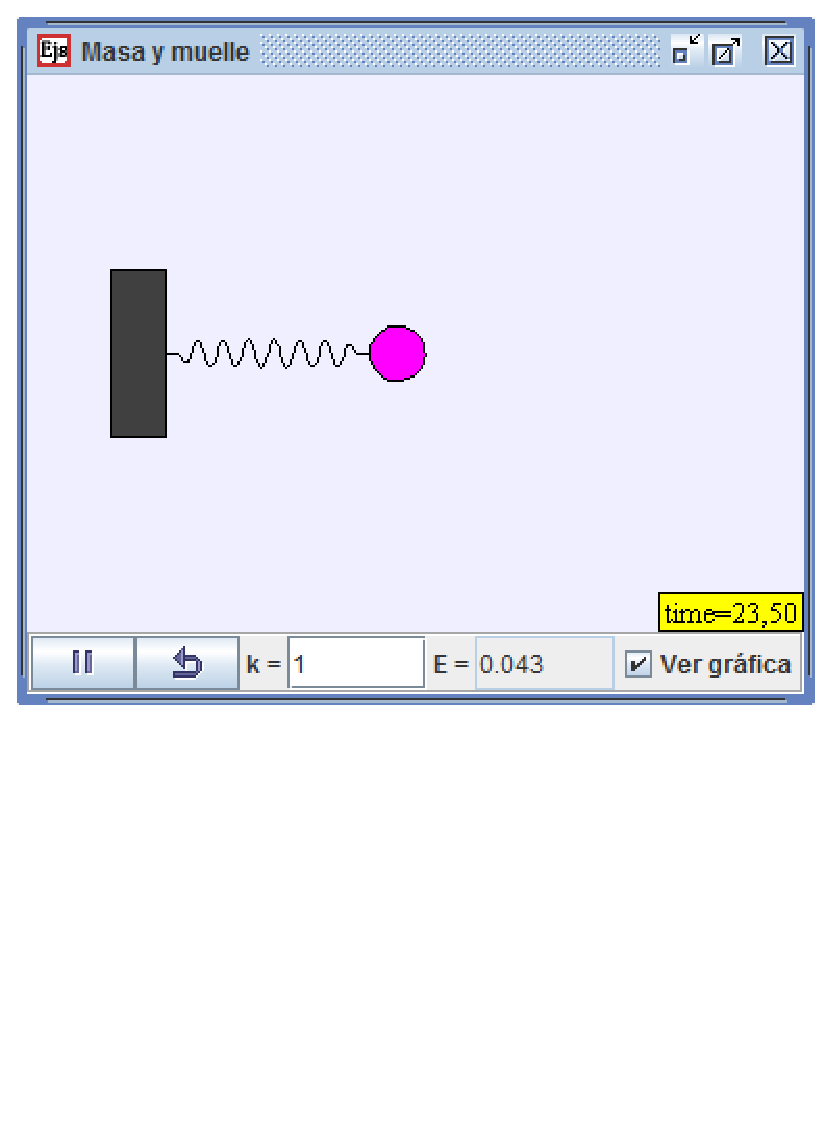
\includegraphics[scale=\scale]{02EjsIntro/images/ModifyRunning1.eps}}
  \subfigure{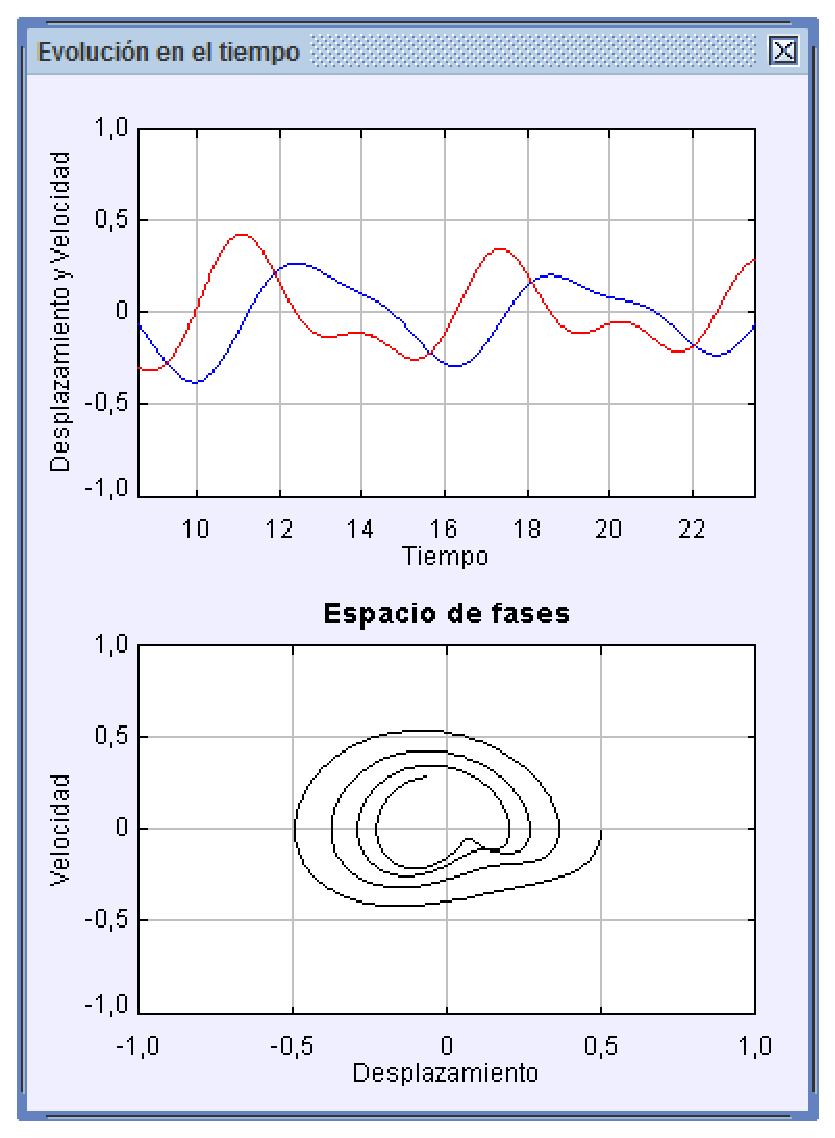
\includegraphics[scale=\scale]{02EjsIntro/images/ModifyRunning2.eps}}
  \caption{The modified simulation. The dialog includes now both a time and a phase-space plot.}
  \label{fig:02EjsIntro/ModifyRunning}
\end{figure}

To finish our view, select the \code{Field} element icon, 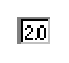
\includegraphics[scale=\linescale]{images/Elements/ParsedField.eps}, on the \lit{Input and output} subgroup of the \lit{Interface} palette. Click three times with the magic wand on the element named \code{fieldsPanel} within the \lit{Tree of Elements} to create three new elements. Name these elements, \code{bField}, \code{amplitudeField}, and \code{frequencyField}. The \code{fieldsPanel} is a simple panel that is designed to hold other interface elements and has been configured (see its properties) to organize its children in three columns. Edit the properties of the new \code{Field} elements so that they are bound to \code{b}, \code{amplitude}, and \code{frequency} variables. For example, edit the \code{bField} properties table as shown in Figure~\ref{fig:02EjsIntro/ModifyField}. The connection to the \code{b} variable is established using the \code{Variable} property.  Click on the second icon to the right of the property field, 
\includegraphics[scale=\linescale]{images/link.eps}, and choose the correct variable. The variable list shows all model variables which can be used to set the property field. The \code{Format} property indicates the prefix and the number of decimal digits with which to display the value of the variable. Repeat this process for the \code{amplitudeField} and \code{frequencyField} properties.

\begin{figure}[htb]
    \centering
  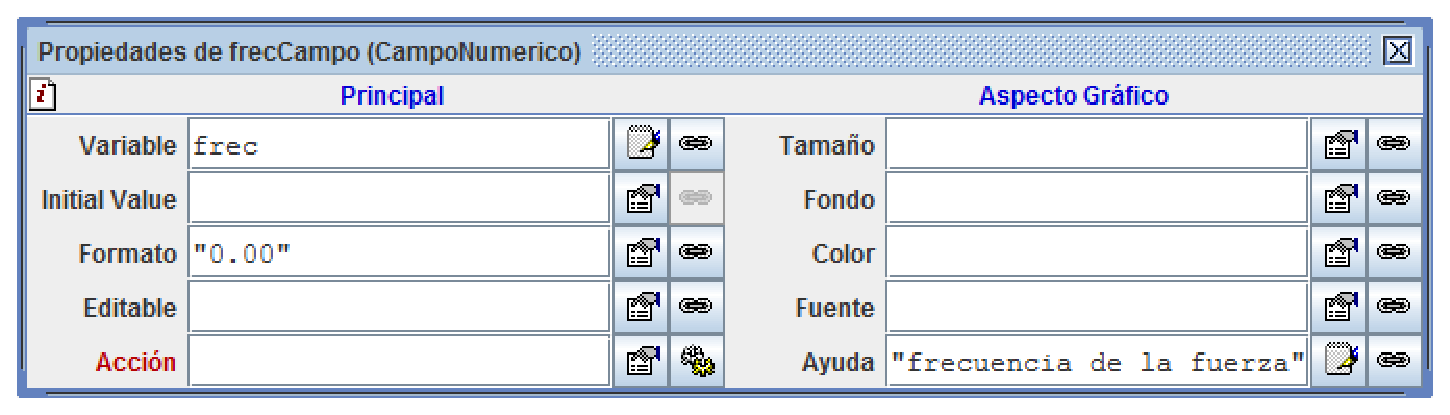
\includegraphics[scale=\scale]{02EjsIntro/images/ModifyField.eps}
    \caption{The table of properties for the \code{bField} element.}
    \label{fig:02EjsIntro/ModifyField}
\end{figure}

\subsection{Changing the description}\label{section:02ModifyingDescription}

Now that we have changed the model and the view, we should modify the description pages of our simulation. Go to the \lit{Description} workpanel and right-click on the tab of the first page, the one labeled \code{Introduction}, to display the popup menu for this page. Select the \lit{Edit/View this page} option. The description page will change to edit mode, as shown in Figure~\ref{fig:02EjsIntro/ModifyHTML}, and a simple editor appears that provides direct access to common HTML features.

If you prefer your own editor, you can copy and paste HTML fragments from your editor into the \ejs\ editor. Authors who know HTML syntax can enter tagged (markup) text directly by clicking the source icon, 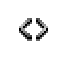
\includegraphics[scale=\linescale]{02EjsIntro/images/SourceHK.eps}, in the tool bar.  You can even import entire HTML pages into \ejs\ by right-clicking on a tab in the workpanel.


\begin{figure}[htb]
    \centering
  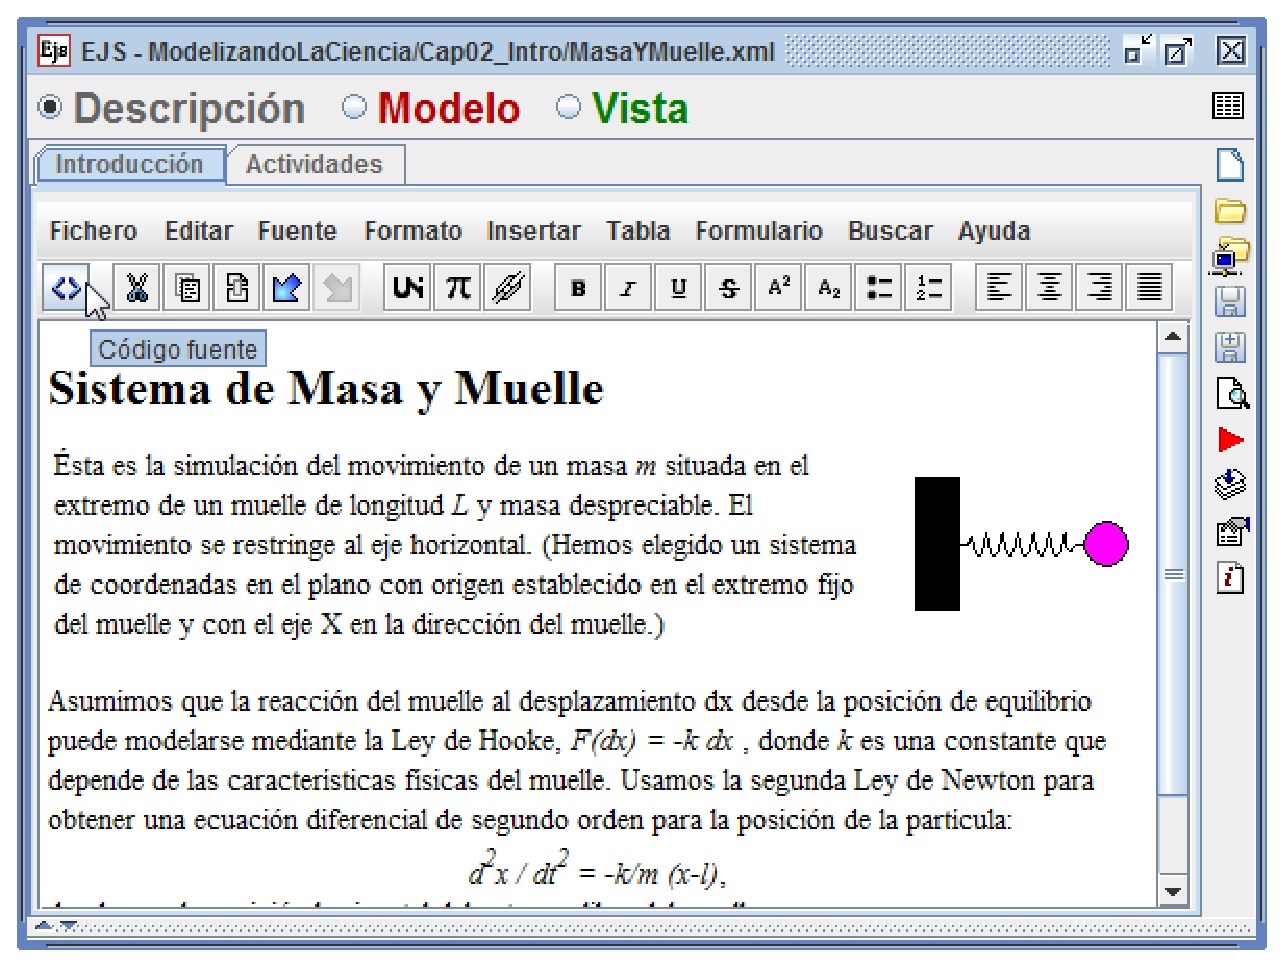
\includegraphics[scale=\scale]{02EjsIntro/images/ModifyHTML.eps}
    \caption{The HTML editor of \ejs. The cursor points to the icon that switches the editor into source code edition mode.}
    \label{fig:02EjsIntro/ModifyHTML}
\end{figure}

Edit the description pages as you find convenient. At least change the discussion of the model to include the damping and driving forces. When you are done, save the new simulation with a different name. For this, click on the \lit{Save As} icon of \ejs' taskbar, \includegraphics[scale=\linescale]{images/saveas.eps}, and, when prompted, enter a new name for your simulation's XML file. Our modified simulation is stored in the \file{MassAndSpringComplete.xml} file in the \file{Simulations} directory for this chapter.

% -----------------------------------------------------
\section{Conclusion}\label{section:02Review}
% -----------------------------------------------------

This book is about modeling and using these models to study and display a wide range
of natural phenomena, from the simple to the very complex. An appropriate way to conduct these studies is to use
computer simulations, that is to program a computer to successively obtain numerical data from our models as they advance
in time, and to display this data in a form humans can easily understand.

\Ejs\ is a modeling and authoring tool expressly devoted to this task. It has been designed to let us work at a high
conceptual level, concentrating most of our time in the scientific aspects of our simulation, and asking the computer
to automatically perform all other necessary but easily automated tasks.
%\ejs\ structures the authoring process in three parts: creating a description, specifying the model, and building the view for the simulation. Each task has a dedicated workpanel that provides the needed functionality. The description workpanel is used to create a set of multimedia HTML pages which provide the necessary narrative to put the model into context. These pages are displayed from within \ejs\ itself, but also when we distribute the simulation in form of a Java applet or within a Launcher package. Creating the model is one of our main tasks, and \ejs\ organizes the process by providing a series of panels that we edit, left to right, to complete the specification: declaration and initialization of variables, evolution pages, constraints (fixed relationships among variables), and custom code. Each panel has specialized capabilities.  The ODE editor stands out and we will see how advanced this editor is when we model many-particle ensembles with arrays. Finally, building the view is made easier by the use of off-the-shelf, ready to use view elements, of which there are many different types, each one specialized for a given visualization or input task. These elements have properties that can be edited to give them either constant or dynamic values that change according to the evolution of the model. We can use these elements to build views whose effectiveness and sophistication rival the work of a professional programmer. Once this high-level work is done, a single mouse click starts the internal engine that will generate a fully dynamic, interactive simulation from our specifications.
Bear in mind that every tool, including \Ejs, has a learning curve. We have made this curve as smooth as possible by carefully designing the \ejs\ interface and by introducing its features progressively. The first part of the book contains a series of detailed examples which familiarize you with the modeling capabilities of \ejs\ and with the most frequently used view elements. The second part of the book is devoted to advanced examples, and puts more emphasis on the scientific content of the models and their behavior. Finally, the appendices cover additional features such as a basic review of Java programming and guidelines that will help you through the unavoidable moment when you make your first programming mistakes.

Modeling is both a science and an art. This book gives you a solid starting point in the science, a coverage of the techniques required by the art, and examples that are useful in professional practice. Always with a bias on modeling and what models tell us about the scientific phenomena being discussed.


% -----------------------------------------------------
\section{Projects}\label{section:02Projects}
% -----------------------------------------------------

\subsection*{Project 1}
Add a third plotting panel to the dialog window of the \file{MassAndSpringComplete.xml} simulation that will display the time evolution of the energies.

\subsection*{Project 2}
Modify the model of the mass and spring simulation to consider motion \emph{not} restricted to the horizontal direction.  Assume that there is a vertical restoring force $f_y=-k' y$. Modify the simulation to allow the user to specify the Hooke's law constant $k'$ in the $y$-direction as well as and the initial conditions in both directions. Describe the motion produced without a driving force but under different initial conditions.

Add a second driving force in the Y direction of the form $F_2(t)=A_2\,\sin(\omega_2\, t + \phi)$ ($\phi$ is a phase difference between both driving forces) and describe the types of motion.

\subsection*{Project 3}
If you feel confident enough, try to create a similar simulation as the one described in this chapter for a non-linear simple pendulum whose second-order differential equation is:
\begin{equation}
  \frac{d^2\theta}{dt^2} = -\frac{g}{l} \sin (\theta).
\end{equation}
\noindent $\theta$ is the angle of the arm of the pendulum with the vertical, $g$ is the acceleration due to gravity, and $l$ is the arms's length. Hint: use constraints to compute the $x$ and $y$ position of the pendulum bob using the equations:
\begin{eqnarray*}
   x   &=&  l \, \sin (\theta) \\
   y   &=& -l \, \cos (\theta).
\end{eqnarray*}

